\documentclass{standalone}
\usepackage{config}
\usetikzlibrary{patterns, calc}

\begin{document}
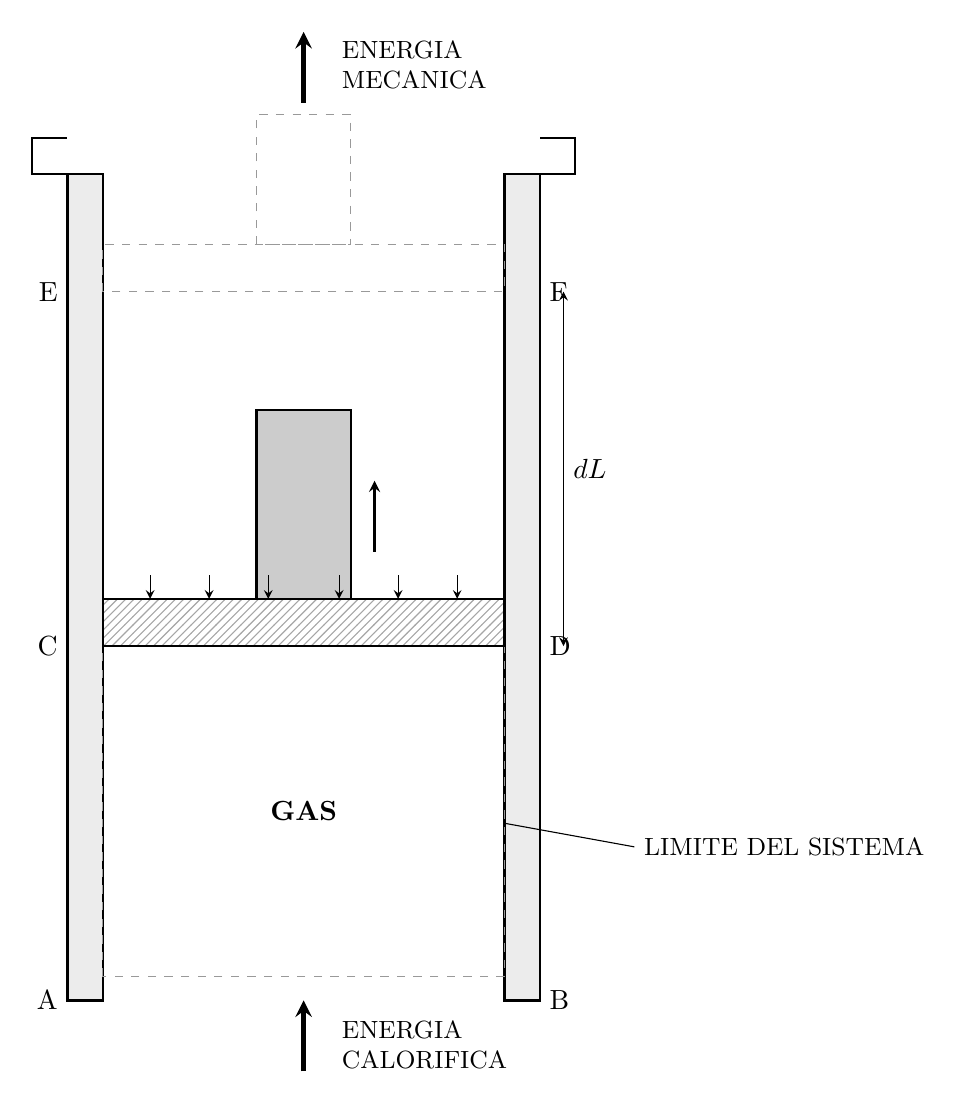
\begin{tikzpicture}[scale=1.5, >=stealth]

    % --- Definición de Estilos ---
    \tikzset{
        wall/.style={draw, thick, fill=gray!15},
        pistonhead/.style={draw, thick, pattern=north east lines, pattern color=gray!70},
        ghost/.style={draw, dashed, thin, gray!80},
        labelnode/.style={font=\small}
    }

    % --- 1. Paredes del Cilindro ---
    \draw[wall] (0,0) rectangle (0.3, 7);
    \draw[wall] (3.7,0) rectangle (4, 7);
    % Topes superiores
    \draw[thick] (0,7) -- (-0.3,7) -- (-0.3,7.3) -- (0,7.3);
    \draw[thick] (4,7) -- (4.3,7) -- (4.3,7.3) -- (4,7.3);

    % --- 2. Límite del Sistema (GAS) ---
    \draw[ghost] (0.3,0.2) rectangle (3.7,3);
    \node at (2, 1.6) {\textbf{GAS}};
    \draw[thin] (3.7, 1.5) -- (4.8, 1.3) node[right, labelnode] {LIMITE DEL SISTEMA};

    % --- 3. Pistón y Vástago (Posición Actual) ---
    \draw[pistonhead] (0.3,3) rectangle (3.7, 3.4);
    \draw[thick, fill=gray!40] (1.6, 3.4) rectangle (2.4, 5);
    
    \foreach \x in {0.7, 1.2, 1.7, 2.3, 2.8, 3.3} {
        \draw[->, thin] (\x, 3.6) -- (\x, 3.4);
    }
    \draw[->, thick] (2.6, 3.8) -- (2.6, 4.4);

    % --- 4. Pistón y Vástago (Posición Fantasma) ---
    \draw[ghost] (0.3,6) rectangle (3.7, 6.4);
    \draw[ghost] (1.6,6.4) rectangle (2.4, 7.5);

    % --- 5. Cotas y Etiquetas ---
    \node[left] at (0,0) {A};
    \node[right] at (4,0) {B};
    \node[left] at (0,3) {C};
    \node[right] at (4,3) {D};
    \node[left] at (0,6) {E};
    \node[right] at (4,6) {F};

    \draw[<->, thin] (4.2, 3) -- (4.2, 6) node[midway, right] {$dL$};

    % --- 6. Flujos de Energía (Ajustados a la derecha) ---
    % Energía Calorífica (Base)
    \draw[->, ultra thick] (2, -0.6) -- (2, 0);
    \node[right, font=\small] at (2.1, -0.4) {\begin{tabular}{l} ENERGIA \\ CALORIFICA \end{tabular}};

    % Energía Mecánica (Tope)
    \draw[->, ultra thick] (2, 7.6) -- (2, 8.2);
    \node[right, font=\small] at (2.1, 7.9) {\begin{tabular}{l} ENERGIA \\ MECANICA \end{tabular}};

\end{tikzpicture}
\end{document}